\documentclass[reprint,superscriptaddress,amsmath,amssymb,aps,prb,longbibliography]{revtex4-2}
\usepackage[utf8]{inputenc}
\usepackage{dcolumn}
\usepackage{bm}% bold math
\usepackage{graphicx}
\usepackage{amsmath}
\usepackage{amssymb}
% \usepackage[section]{placeins}
\usepackage{placeins}
\usepackage{float}
\usepackage{color, xcolor}
\usepackage[normalem]{ulem}
\usepackage{newunicodechar}
\newunicodechar{）}{)}
\usepackage{soul}
\soulregister\cite7
\soulregister\ref7


\renewcommand{\topfraction}{0.9}
\renewcommand{\bottomfraction}{0.8}
\renewcommand{\textfraction}{0.07}
\renewcommand{\floatpagefraction}{0.75}
\renewcommand{\dbltopfraction}{0.9}
\renewcommand{\dblfloatpagefraction}{0.7}
\setcounter{topnumber}{3}
\setcounter{bottomnumber}{2}
\setcounter{totalnumber}{4}
\setcounter{dbltopnumber}{3}

\begin{document} 
\flushbottom
\title{Interaction-driven altermagnetism in the checkerboard Hubbard model}
\author{Rana Imran Mushtaq}
% \thanks{These authors contributed equally.}
\affiliation{School of Science, Harbin Institute of Technology, Shenzhen, 518055, China}
\affiliation{Shenzhen Key Laboratory of Advanced Functional Carbon Materials Research and Comprehensive Application, Shenzhen 518055, China.}

% \author{Ji Liu}
% \thanks{These authors contributed equally.}
% \affiliation{School of Science, Harbin Institute of Technology, Shenzhen, 518055, China}
% \affiliation{Shenzhen Key Laboratory of Advanced Functional Carbon Materials Research and Comprehensive Application, Shenzhen 518055, China.}

% \author{Yinlong Li}
% \affiliation{School of Science, Harbin Institute of Technology, Shenzhen, 518055, China}
% \affiliation{Shenzhen Key Laboratory of Advanced Functional Carbon Materials Research and Comprehensive Application, Shenzhen 518055, 
% China.}

% \author{Wing Chi Yu}
% \email{wingcyu@cityu.edu.hk}
% \affiliation{Department of Physics, City University of Hong Kong, Kowloon, Hong Kong
% }

% \author{Xiaosen Yang}
% \email{yangxs@ujs.edu.cn}
% \affiliation{Department of Physics, Jiangsu University, Zhenjiang, 212013, China.}

\author{Ho-Kin Tang}
\email{denghaojian@hit.edu.cn}
\affiliation{School of Science, Harbin Institute of Technology, Shenzhen, 518055, China}
\affiliation{Shenzhen Key Laboratory of Advanced Functional Carbon Materials Research and Comprehensive Application, Shenzhen 518055, China.}

\begin{abstract}
Altermagnets combine antiferromagnetic compensation with a momentum-dependent, spin-split band structure of definite $d$-wave symmetry, yet most microscopic studies impose this splitting through spin-dependent hopping or treat it within mean-field theory. We study altermagnetism that emerges from electronic correlations in a
spin-independent single-band Hubbard model on the anisotropic checkerboard (planar-pyrochlore) lattice, using constrained-path and determinant quantum Monte Carlo benchmarked against exact diagonalization. The geometric diagonal anisotropy $\delta$ turns the interaction-driven N\'eel order into an altermagnet whose spin splitting has $d_{xy}$ symmetry and scales as the product $M\delta$ of the ordered moment $M$ and the anisotropy, vanishing when either is absent. In the filling--anisotropy plane, long-range N\'eel order is confined to the
vicinity of half-filling, while doping yields short-range incommensurate correlations. Because the altermagnetic form factor is fixed by the lattice geometry, it is $d_{xy}$ here rather than the $d_{x^2-y^2}$ of
square-lattice models, which implies a distinct symmetry channel for interaction-driven pairing. These results identify the checkerboard Hubbard model as a minimal, unbiased setting for interaction-driven altermagnetism.
\end{abstract}

\maketitle

\section{INTRODUCTION}
\label{Introduction}


\section{Model and Method}
\label{Model and Method}
\subsection{Model Hamiltonian}
\label{Combined model}

\subsection{Magnetic observables}
\label{sec:observables}

\begin{figure*}
    \centering
    
\includegraphics[width=0.8\textwidth]{figures/1_dnk.png}
    \caption{(a) Schematic diagram of the checkerboard Hubbard model with isotropic nearest-neighbor hopping $t$ and anisotropic diagonal hopping $t_\pm = t' \pm \delta$ on alternating plaquettes. (b)--(d) Mean-field momentum-resolved spin polarization $\Delta n(\mathbf{k})$ for $\delta = 0,\,0.2,\,0.4$. The polarization vanishes at $\delta = 0$ and forms a $d_{xy}$ pattern that grows with $\delta$, so the ordered state is an altermagnet with zero net moment. Parameters are $t = 1$ and $t' = -0.3$. The ordered moment $M$ and chemical potential take representative mean-field values.}
    \label{fig:model}
\end{figure*}

\section{Noninteracting Electronic Structure}
\label{sec:noninteracting}

\begin{figure*}
  \centering
  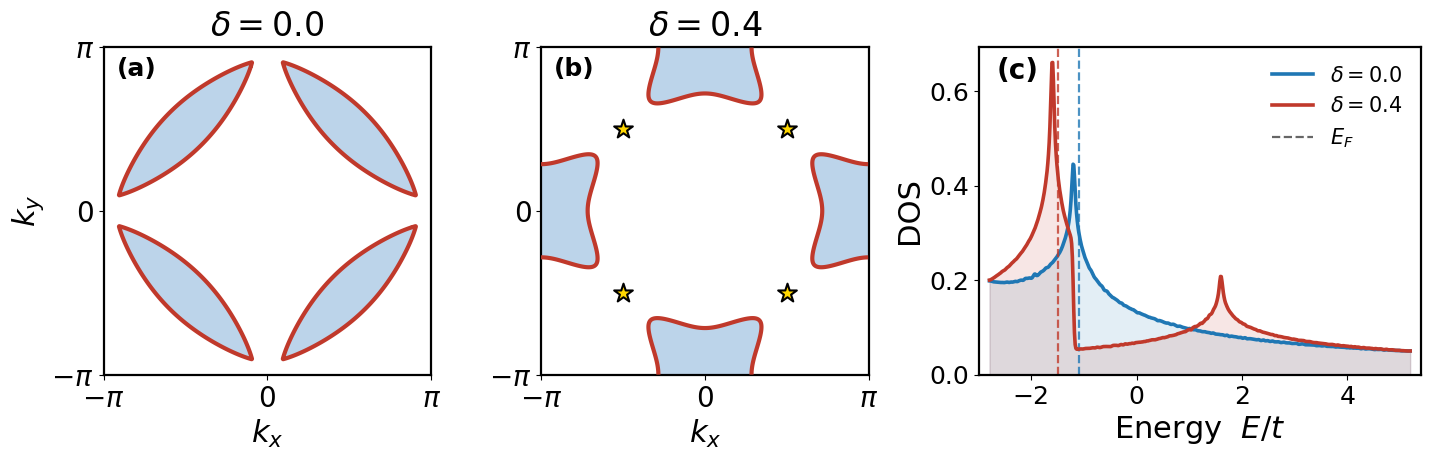
\includegraphics[width=0.8\textwidth]{figures/2_vhs_dos.png}
  \caption{Non-interacting single-particle structure of the checkerboard model ($t=1$, $t'=-0.3$, $n=0.8$). (a),(b) Fermi surface for $\delta=0$ and $\delta=0.4$. White is the occupied Fermi sea, light blue the empty states, the red curve is the Fermi surface, and gold stars mark the van Hove saddle points. Increasing $\delta$ drives a Lifshitz reconstruction and moves the saddle points close to the Fermi level. (c) Density of states for the same two values of $\delta$, with dashed lines at the Fermi level. The van Hove saddle points of (a),(b) appear here as peaks. Increasing $\delta$ shifts the lower-band peak from $E=4t'$ to $E=-4\delta$ and raises the density of states near the Fermi level.}
  \label{fig:vhsdos}
\end{figure*}

\begin{figure}[t]
  \centering
  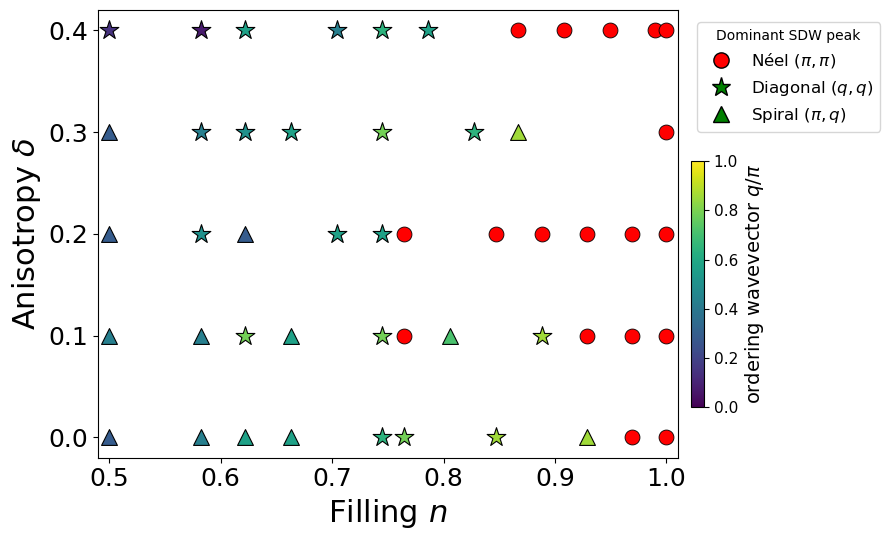
\includegraphics[width=\columnwidth]{figures/3_phase_diagram.png}
  \caption{Distribution of the dominant $S^{z}(\mathbf{k})$ peak location in the $(n,\delta)$ plane for an $L=14$ lattice at $U=4$ and $t'=-0.3$. Each point is labeled by the ordering vector $\mathbf{Q}$. Three correlations are identified as N\'eel order at $(\pi,\pi)$ (red circles), spiral correlation at $(\pi,q)/(q,\pi)$ (triangles), and diagonal correlation at $(q,q)$ (stars). The color encodes the wavevector $q/\pi$. N\'eel correlations dominate near half filling for all $\delta$, while doping drives the system toward spiral and diagonal correlations.}
  \label{fig:phase_diagram}
\end{figure}

\begin{figure}[t]
  \centering
  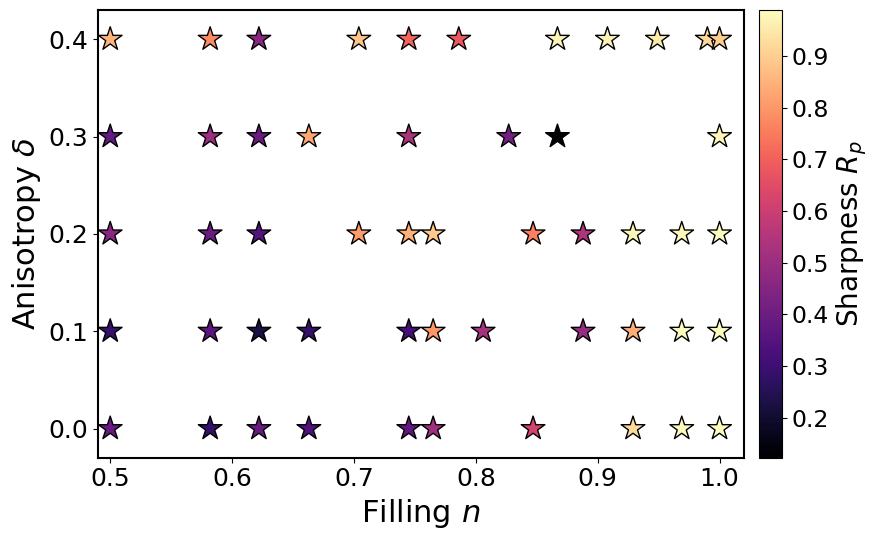
\includegraphics[width=\columnwidth]{figures/4_rp.png}
  \caption{Sharpness index $R_{p}$ of the dominant $S^{z}(\mathbf{k})$ peak in the $(n,\delta)$ plane for an $L=14$ lattice at $U=4$ and $t'=-0.3$. A large $R_{p}$ marks a sharp peak and long-range magnetic order, while a small $R_{p}$ marks a broad peak and short-range correlation. The sharpest peaks appear near half filling, consistent with the N\'eel order, and $R_{p}$ decreases upon doping.}
  \label{fig:rp}
\end{figure}

\begin{figure*}[t]
  \centering
  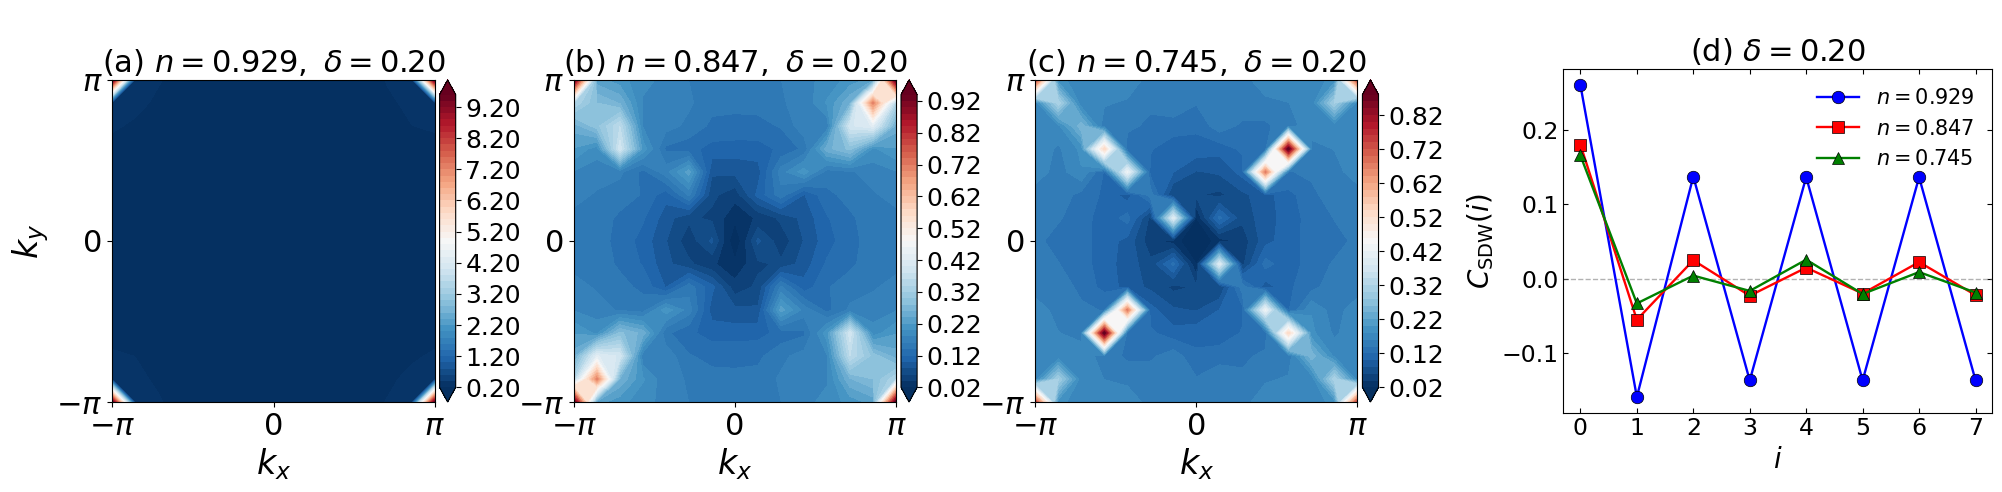
\includegraphics[width=0.8\textwidth]{figures/5_sdw.png}
  \caption{Momentum-space and real-space spin correlation at fixed anisotropy $\delta=0.20$ for three fillings. (a)--(c) Spin structure factor $S^{z}(\mathbf{k})$ for $n=0.929$, $0.847$, and $0.745$. As the filling decreases, the dominant peak moves from $(\pi,\pi)$ to $(\pi,q)/(q,\pi)$ and then to $(q,q)$. The peak intensity is largest at $n=0.929$, where $S^{z}(\pi,\pi)$ is more than an order of magnitude stronger than at the doped points. (d) Real-space correlation $C_{\mathrm{SDW}}(i)$ for the same three fillings. At $n=0.929$ the correlation shows a robust staggered structure that persists over the accessible distances, while at lower filling it decays rapidly.}
  \label{fig:sdw}
\end{figure*}

\begin{figure}[t]
  \centering
  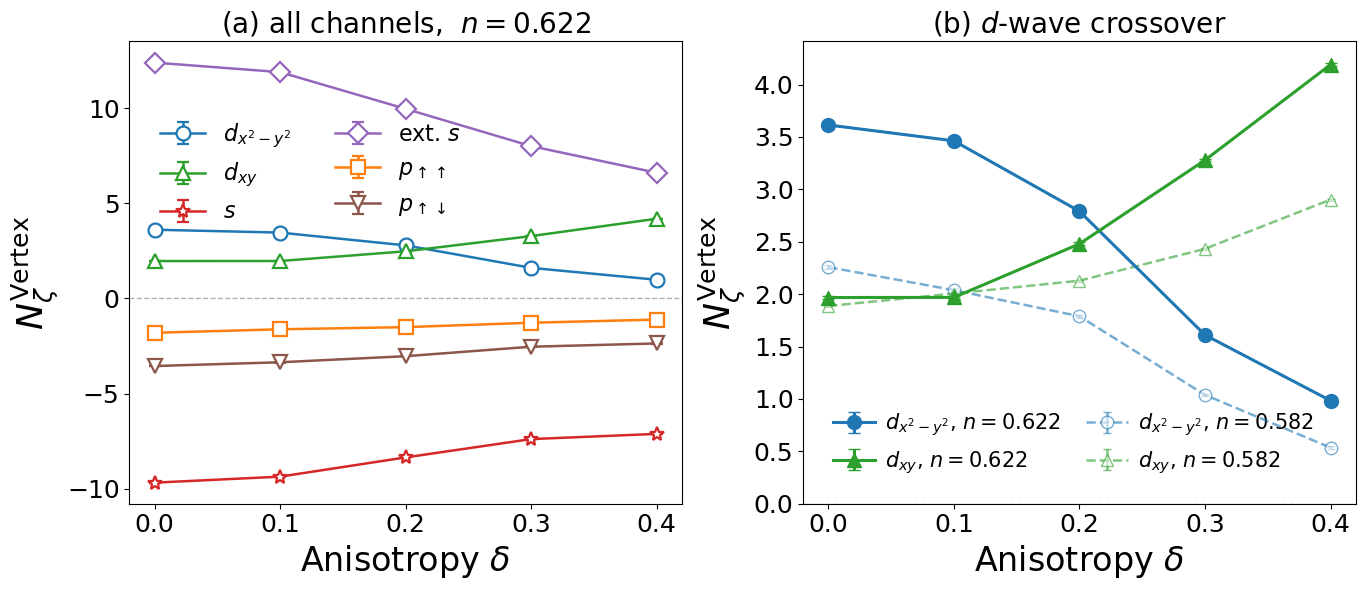
\includegraphics[width=\columnwidth]{figures/6_pairing.png}
  \caption{Equal-time connected pairing vertex $N^{\mathrm{Vertex}}_{\zeta}$ as a function of the anisotropy $\delta$ at $U=4$, $L=14$. (a) All pairing channels at fixed filling $n=0.622$. The on-site $s$ channel is strongly negative, reflectin the on-site Coulomb repulsion, and the extended $s$ channel is the largest. (b) The two $d$-wave channels for $n=0.622$ (solid) and $n=0.582$ (dashed). As $\delta$ increases the $d_{x^2-y^2}$ vertex decreases and the $d_{xy}$ vertex increases, and the two cross near $\delta\approx0.1$ to $0.2$. Among the unconventional pairing channels the checkerboard anisotropy selects $d_{xy}$.}
  \label{fig:pairing_crossover}
\end{figure}

\begin{figure*}[t]
  \centering
  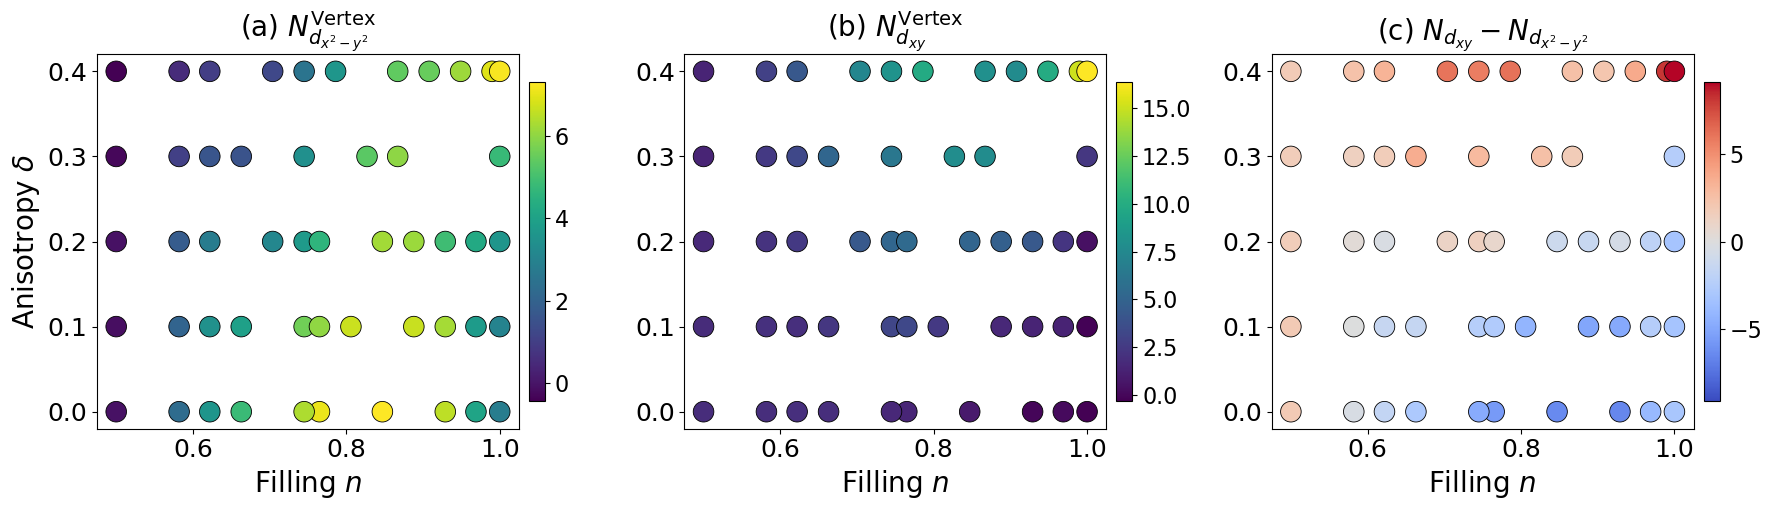
\includegraphics[width=0.8\textwidth]{figures/7_pairing_pd.png}
  \caption{Equal-time connected pairing vertex in the filling--anisotropy $(n,\delta)$ plane at $U=4$, $L=14$. (a) The $d_{x^2-y^2}$ vertex is largest at small $\delta$. (b) The $d_{xy}$ vertex is largest at large $\delta$. (c) The difference $N_{d_{xy}}-N_{d_{x^2-y^2}}$, positive (red) where $d_{xy}$ dominates and negative (blue) where $d_{x^2-y^2}$ dominates. The dominant $d$-wave pairing symmetry changes from $d_{x^2-y^2}$ to $d_{xy}$ across the plane.}
  \label{fig:pairing_pd}
\end{figure*}

\begin{figure}[t]
  \centering
  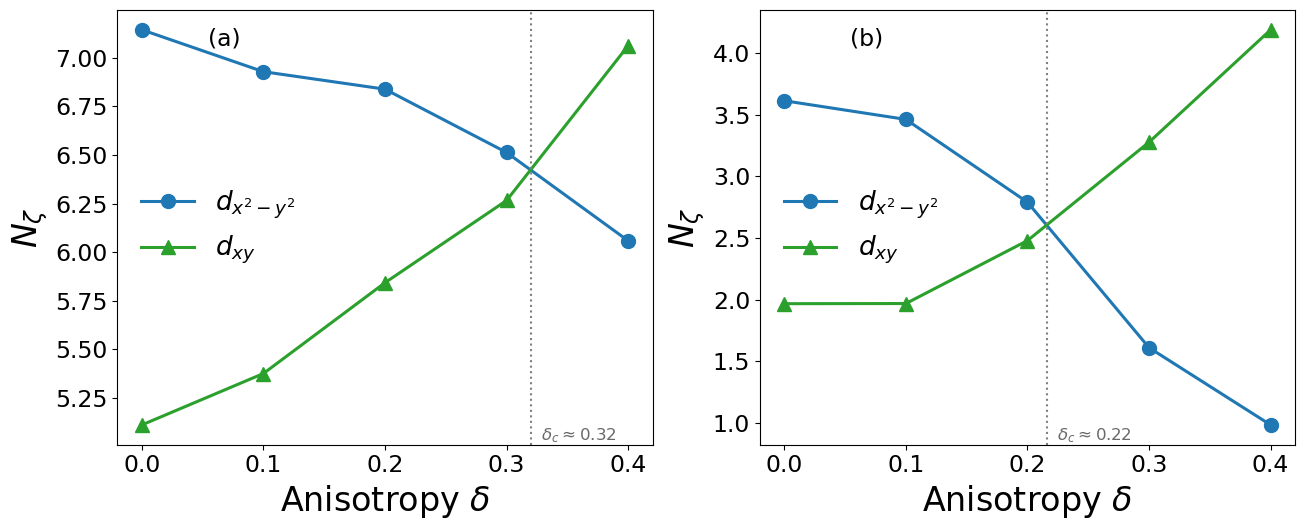
\includegraphics[width=\columnwidth]{figures/8_d_crossover.png}
  \caption{Decomposition of the $d$-wave pairing correlations at $n=0.622$ into (a) Unpair and (b) Vertex. The unpair varies weakly with $\delta$ and the two $d$-wave channels cross near $\delta\approx0.32$, while the connected vertex shows a sharper crossover near $\delta\approx0.22$ with the $d_{x^2-y^2}$ channel strongly suppressed. The lattice geometry sets the direction of the crossover and the on-site repulsion drives and sharpens it.}
  \label{fig:bare_vs_vertex}
\end{figure}

\subsection{Momentum-dependent spin splitting and band reconstruction}

\subsection{Van Hove singularities}
\label{VHS_distribution}


\section{Evolution of Magnetic Correlations}
\label{magnetic_correlations}


\subsection{Phase diagram of the NN altermagnetic model}
\label{sec:NN_phase}


\subsection{Phase diagram of the combined model}
\label{sec:combined_phase}


\subsection{Spatial range of the magnetic correlations}
\label{sec:Rp_real}


\subsection{Magnetic correlations near and away from half filling}
\label{sec:regimes}


\section{Conclusion}

\section*{Acknowledgment}
This work is supported by the Shenzhen Fundamental Research Program (No.~JCYJ20250604145655074), and Shenzhen Key Laboratory of Advanced Functional Carbon Materials Research and Comprehensive Application (Grant No. ZDSYS20220527171407017).


\appendix
\section*{Appendix A: Noninteracting electronic structure of the NN model}
\label{app:noninteracting}

\section*{Appendix B: Finite-size dependence of the combined model phase diagram}
\label{app:finite_size}

%\FloatBarrier


% \bibliographystyle{apsrev4-2}
\bibliography{references}
\end{document}
